\begin{exo}
	On fait tourner la roue ci-dessous dont tous les secteurs angulaires sont de même mesure.

	\begin{center}
		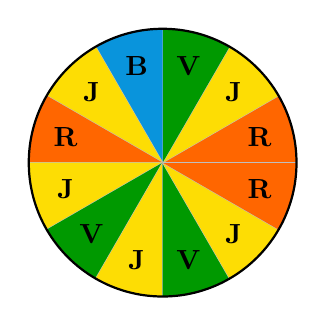
\begin{tikzpicture}[scale=0.85]
			\def\sectors{ 1/{orange!80!red}/R, 2/{yellow!80!orange}/J, 3/{green!60!black}/V, 4/{cyan!80!blue}/B, 5/{yellow!80!orange}/J, 6/{orange!80!red}/R, 7/{yellow!80!orange}/J, 8/{green!60!black}/V, 9/{yellow!80!orange}/J, 10/{green!60!black}/V, 11/{yellow!80!orange}/J, 12/{orange!80!red}/R }
			\foreach \i/\col/\text in \sectors {
			\fill[\col] (0,0) -- ({(\i-1)*30}:2) arc ({(\i-1)*30}:{\i*30}:2) -- cycle;
			\draw[gray!50] (0,0) -- ({\i*30}:2);
			\node at ({(\i-0.5)*30}:1.5) {\textbf{\text}};
			}
			\draw[thick] (0,0) circle (2);
		\end{tikzpicture}
	\end{center}

	Reproduire et compléter le tableau ci-dessous.
	\begin{center}
		\def\arraystretch{1.5}
		\begin{tabular}{|c|c|c|c|c|} \hline
			\cellcolor{gray!30}Couleur     & Bleu & Rouge & Vert & Jaune \\ \hline
			\cellcolor{gray!30}Probabilité &      &       &      &       \\ \hline
		\end{tabular}
	\end{center}
\end{exo}
